\section{Ticket 2: Булевские значения, чёрчевские нумералы, упорядоченные пары,
  алгебраические типы. Нормальный и аппликативный порядок редукции.
  Бета-эквивалентность и Y-комбинатор. Парадокс Карри.}
\label{sec-3}
\subsection{Булевские значения}
\label{sec-3-1}
Значения Булевской логики можно определить так:

\begin{align*}
T &= \lambda x . \lambda y . x \\
F &= \lambda x . \lambda y . y
\end{align*}

Очевидно это просто два проектора. Определим несколько интересных операций в
булевской логике:

\begin{align*}
ifThenElse &= \lambda A . \lambda P . \lambda Q . A P Q \\
and &= \lambda A . \lambda B . A B F \\
not &= \lambda A . A F T \\
xor &= \lambda A . \lambda B . A (not B) B
\end{align*}

\subsection{Пары}
\label{sec-3-2}
Пара и её проекторы определяются следующим образом:
\begin{align*}
\langle A, B \rangle &= \lambda x . x A B \\
\pi_1 &= \lambda x . \lambda y . x \\
\pi_2 &= \lambda x . \lambda y . y \\
fst &= \lambda p . p \pi_1 \\
snd &= \lambda p . p \pi_2
\end{align*}

\subsection{Чёрчевские нумералы}
\label{sec-3-3}

Определим $n$-разовое приминение функции $f$ как:
\begin{align*}
f^0(A) &= A \\
f^{n+1}(A) &= f(f^n(A))
\end{align*}

Тогда пусть $\bar{n}$ будет $n$-ым Чёрчевским нумералом, если:
\begin{equation}
\bar{n} = \lambda f . \lambda x . f^n(x)
\end{equation}

Наблюдение: $\bar{0} = F$.

Определим арифметику на Чёрчевских нумералах:
\begin{align*}
isZero &= \lambda a . a \lambda x . F) T \\
inc &= \lambda a . \lambda f . \lambda x . f (a f x) \\
plus &= \lambda a . \lambda  b . \lambda f . \lambda x . a f (b f x) \\
mul &= \lambda a . \lambda b . \lambda f . a (b f) \\
pow &= \lambda a . \lambda b . b a
\end{align*}

Понимать их следует так: $isZero$ значит, что если хоть раз будет применено $f$, 
то число не ноль, иначе ноль. $inc$ значит, что нужно ещё
один раз применить $f$ к $a$. $plus$ значит, что нужно просто передать значение
$a$ как начальное значение $b$.

Также с помощью пар можно реализовать вычитание. Начнём с $\langle 0, 0 \rangle$ и будем
поддерживать пару $\langle n, n - 1 \rangle$, пока $n$ не окажется равным $a$.
\begin{equation}
dec = \lambda a . snd (a (\lambda p . \langle inc (fst p); fst p \rangle ) \langle 0, 0 \rangle )
\end{equation}

\subsection{Алгебраические типы}
\label{sec-3-4}

\myworries{Алгебраический тип -- любой сложный тип, состоящий из более простых
  типов}

\subsection{Нормальный и аппликативный порядок редукции}
\label{sec-3-5}
Рассмотрим способы редуцирования терма
\begin{align*}
v &\not\rightarrow_\beta \\
\lambda x . M &\rightarrow_\beta \lambda x . M' \\
M N &\rightarrow_\beta M' N \\
M N &\rightarrow_\beta M N'
\end{align*}
Получается, что выбор в редуцировании возникает только в аппликации. Тогда
определим эти порядки редукции:

Нормальный порядок редукции -- редукция, при которой первым делом сокращается
редекс $(\lambda x . M) N$.

Аппликативный порядок редукции -- редукция, при которой первым делом сокращается
$N$, а затем уже редекс $(\lambda x . M) N'$.

\subsection{$\beta$-эквивалентность}
\label{sec-3-6}

Бинарное отношение $=_\beta$ над $\Lambda$ определяется индуктивно:

\begin{align*}
M \twoheadrightarrow_\beta N &\Rightarrow M =_\beta N \\
M =_\beta N &\Rightarrow N =_\beta M \\
M =_\beta N, N =_\beta L &\Rightarrow M =_\beta L
\end{align*}

Интуитивно: два терма $M$ и $N$ связаны отношением $=_\beta$, если есть
связывающая их цепочка $\rightarrow_\beta$-стрелок.

Пример: \\
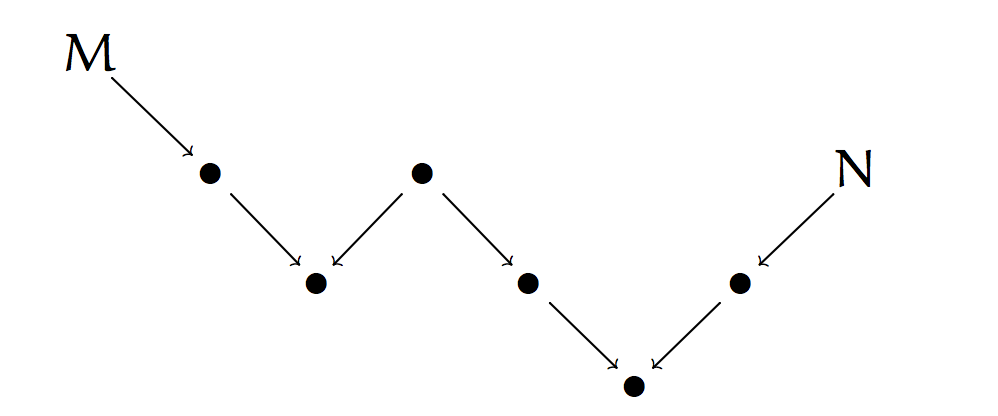
\includegraphics[scale=0.5]{resources/beta_equality.png}

\subsection{Y-комбинатор}
\label{sec-3-7}

\begin{theorem}
Для любого $F$ найдётся такой $X$ (неподвижная точка), что:
\begin{equation}
F X =_\beta X
\end{equation}
\end{theorem}
\begin{proof}
Пусть $W = \lambda x . F (x x)$, а $X = WW$. Тогда $X = WW = (\lambda x . F (x
x)) W = F (W W) = F X$
\end{proof}

\begin{theorem}
Существует комбинатор неподвижной точки $Y = \lambda f . (\lambda x . f (x x))
(\lambda x . f (x x))$ такой, что $\forall F \  F (Y F) = Y F$
\end{theorem}
\begin{proof}
Очевидно если расписать $Y F$
\end{proof}

% \myworries{Возможно стоит сказать о F =_\beta M[f:=F]}

\subsection{Парадокс Карри}

Построим исчисление высказываний на основе язык лямбда выражений. Для этого
добавим к аппликации импликацию ($\supset$), которое будет действовать по
следующим правилам:

\begin{align*}
A =_\beta B &\Rightarrow \ \vdash A \supset B \\
A =_\beta B &\Rightarrow \ \vdash B \supset A \\
\end{align*}

Также мы ожидаем доказуемости следующих свойств:

\begin{align*}
&\vdash \alpha \supset \alpha \\
\alpha \supset \alpha \supset \beta &\vdash \alpha \supset \beta 
\end{align*}

Однако, так построенное исчисление черезчур мощно, о чём свидетельствует
следующее утверждение:

Рассмотрим выражение $F_\alpha \equiv \lambda x. x x \supset \alpha$ 
и выражение $\Phi_\alpha \equiv F_\alpha F_\alpha$.
Нетрудно видеть, что $\Phi_\alpha =_\beta \Phi_\alpha \supset \alpha$.
Тогда: \\

\begin{tabular}{ll}
$\vdash \Phi_\alpha \supset \Phi_\alpha$ & Доказуемое утверждение\\
$\vdash \Phi_\alpha \supset \Phi_\alpha \supset \alpha$ & По определению ($=_\beta$)\\
$\vdash (\Phi_\alpha \supset \Phi_\alpha \supset \alpha) \supset (\Phi_\alpha \supset \alpha)$ & Доказуемое утверждение\\
$\vdash \Phi_\alpha \supset \alpha$ & M.P.\\
$\vdash \Phi_\alpha$ & бета-эквивалентность\\
$\vdash \alpha$ & M.P.
\end{tabular}

Таким образом мы показали, что любое утверждение может быть выведено в данной
системе, т.е. система противоречива.